\documentclass[journal]{IEEEtran}
\usepackage{graphicx}
\usepackage[utf8]{inputenc}
\usepackage{float}
\ifCLASSINFOpdf
\else
\fi
\hyphenation{op-tical net-works semi-conduc-tor}
\begin{document}
\title{SHA-256 PAPER}
\author{Eduard~Torres~Chaves~\IEEEmembership{}
        and~Juan~José~Solano~Quesada~\IEEEmembership{}
\thanks{E. Torres Chaves Computer Engineering student, Instituto Tecnológico de Costa Rica}% <-this % stops a space
\thanks{J.J. Solano Computer Engineering student, Instituto Tecnológico de Costa Rica}% <-this % stops a space
\thanks{}}
\maketitle
\begin{abstract}
Define what's the SHA-256 cryptographic method, what it does and how it works. Emperimentation on how long it takes for the method to generate a result for different input sizes.

\end{abstract}
\begin{IEEEkeywords}hash, cryptographic, bit, logic operation
\end{IEEEkeywords}
\IEEEpeerreviewmaketitle

\section{Introduction}
In this paper we will talk about the study and experimentation of the SHA-256 hash function, is important to know that SHA-256 isn't an encryption algorithm, it is a ‘one-way’ cryptographic function.\ SHA-256 is a member of the SHA-2 family, which was designed by the United States National Security Agency (NSA).\\ It's one of the successor hash functions to SHA-1, but is not much complex.The uses of SHA-256 goes from hash tables, integrity verification, challenge handshake authentication to digital signatures, etc.\\ 
The fact of being a cryptographic hash functions is their collision resistance: nobody should be able to find two different input values that result in the same hash output.\\
SHA-256 creates an 256-bit key (from there comes the name), that make it perfect partner-function for AES(Advanced Encryption Standard) and other's alike.
\section{Methodology}
The chosen model is the qualitative one, because it allows us to use experimentation to obtain the necessary data to reach conclusions about the function, we will make distinct experiments around the Java code of the SHA-256 function, once we finish the tests, we will compare then to know the trend of the function with different sizes of input text and the time spent in "digesting" them.\\heil 
The string list used in the experiments is:
[ "abc","test", "one after one", "Heil Hitler", "today is gonna be a beautiful day", "I don't think you trust\ In my self righteous suicide\ I cry when angels deserve to die!"].\\
In the figure 1, is the result of a python code that counts the number of characters which has each string in the previous list, the difference in numbers of characters is important for the test diversity(the presence of uppercase and lowercase letters should not affect the digesting time). \\
 Next is the Java code (figure 2) that is used in the test realization, the code has a string which is digested and comes out in a byte vector, which is manipulated to be transformed into a readable string.
\begin{figure}[h] 
	\centering 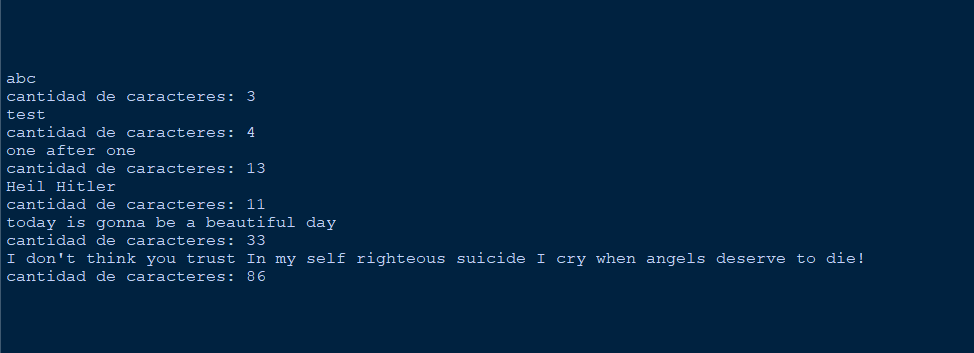
\includegraphics[width=.70\columnwidth]{CantidadDeCaracteres.png}
	\caption{
		\label{fig:samplesetup}
		Result of the character counter in Python
	}
\end{figure}
\begin{figure}[h] 
	\centering 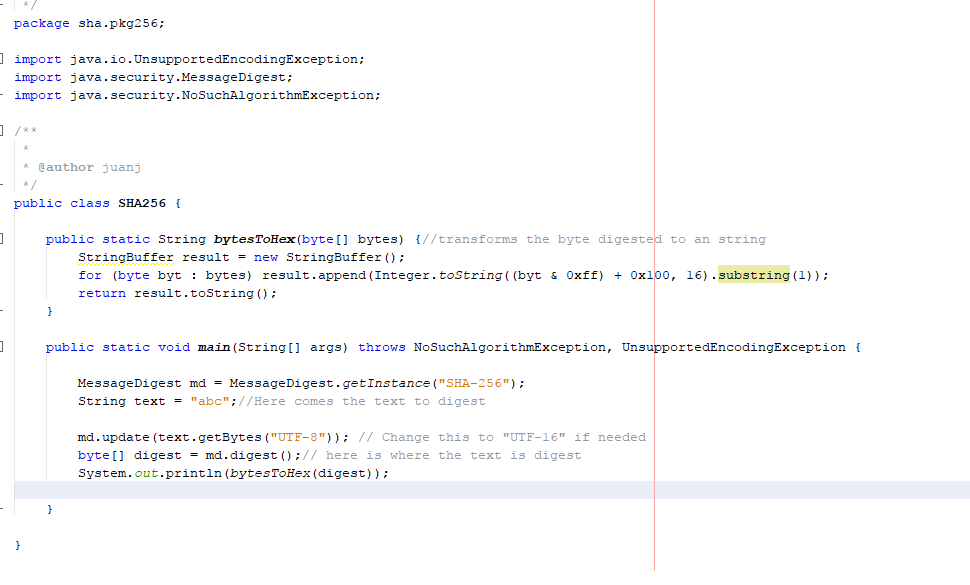
\includegraphics[width=.70\columnwidth]{Sha-256Code.png}
	\caption{
		\label{fig:samplesetup}
		SHA-256 Java Code 
	}
\end{figure}
\section{Experimentation}
The algorithm gets the message from the input and processes it to get the bits of it, then adds a number 1 to the end and appends number 0s to make the message a 512 multiple length and finally the length of the message is appended at the end in 64-bit big-endian format. Then, for every 512 bit chunk a series of logical operations (shown in figure 3) are applied to the first 16 words of the chunk to extend the words across the entire 512 bit segment.
\begin{figure}[H] 
	\centering 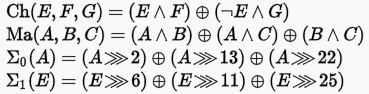
\includegraphics[width=.70\columnwidth]{logic.png}
	\caption{
		\label{fig:samplesetup}
		Logical operations performed to 512 bit chunks
	}
\end{figure}
The complexity used to generate the hash code is $O(2^{64})$ because of the size of the word that divides every chunk, which is 64 bits.\\
Now, we will apply the code to all strings in the already defined list.
\begin{figure}[H] 
	\centering \includegraphics[width=.70\columnwidth]{captura.png}
	\caption{
		\label{fig:samplesetup}
		SHA-256 applied to "abc"
	}
\end{figure}
\begin{figure}[H] 
	\centering 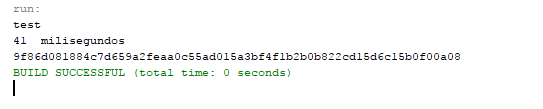
\includegraphics[width=.70\columnwidth]{Code_test.png}
	\caption{
		\label{fig:samplesetup}
		SHA-256 applied to "test"
	}
\end{figure}
\begin{figure}[H] 
	\centering 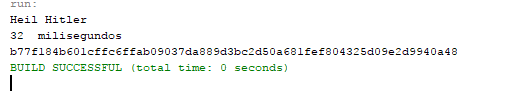
\includegraphics[width=.70\columnwidth]{Code_heil.png}
	\caption{
		\label{fig:samplesetup}
		SHA-256 applied to "Heil Hitler"
	}
\end{figure}
\begin{figure}[H] 
	\centering 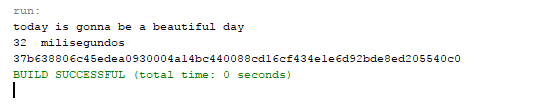
\includegraphics[width=.70\columnwidth]{Code_today.png}
	\caption{
		\label{fig:samplesetup}
		SHA-256 applied to "today is gonna be a beautiful day"
	}
\end{figure}
\begin{figure}[H] 
	\centering 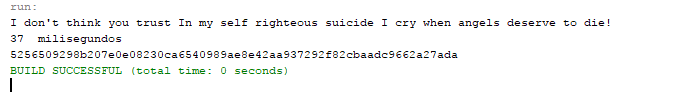
\includegraphics[width=.70\columnwidth]{Code_Long.png}
	\caption{
		\label{fig:samplesetup}
		SHA-256 applied to "I don't think you trust In my self righteous suicide I cry when angels deserve to die!"
	}
\end{figure}

With the above, we can proceed to the data analysis to obtain results.
\section{Results}
With the tests carried out, it is noted that the times to execute or digest the strings, tend to last the same, around 20-40 milliseconds,
of course, these times are affected by the processes that are running the system simultaneously, but the effects of those process are usually minimal on the hash.\\It is worth mentioning that the size or number of characters in the string does not seem to affect the time to digest, as seen in the tests, due to the SHA-256 process to digest the set of bytes that make up the string.\\When seeing the order of the procedure, it coincides with the observed in the times of execution, since the large O is a constant $C$, there should not be times greater than the same $C=2^{64}$.\\With these results, the utility of the SHA-256 function in the algorithms and computational security processes is seen, since it is a fast, relatively simple function and since it is not an encryption method, the possibility of reaching the original string from of the string passed by the SHA-256 function, it is almost null.
\section{Discussion}
This algorithm is pretty complex, that's what makes it a secure way for hashing passwords and other security protocols, since it's a one-way conversion and there's no exact method to get the original input from a hashed result.\\
However there's been experimentation with some attacks in order to retrieve the original message starting from the result, using a differential method causing pseudo-collusions, and this algorithm complexity turned out to be $O(2^{37})$. This means that it makes 37 rounds out of 64, that is what the original algorithm takes, and that's why it doesn't produce an exact answer always.
♣
\section{Conclusions}
It can be concluded that the function SHA-256, is fast and secure, because of what was found in the tests and results given earlier in this document, in comparison with other hash methods, in addition, being a function with a big O of constant type, gives the assurance that it will be a quick result.\\The fact that SHA-256 function always returns a single result of equal size, allows a consistency at the time of use in algorithms and computer systems.\\ Being a ‘one-way’ cryptographic function almost completely eliminates the possibility of being "hacked" or compromised in any way, except for the cases given earlier in the discussion, making it particularly effective in algorithms related to password security or data verification.
\end{document}